\section{Теорія імітостійкості}
\begin{flushright}
\emph{(Автор: Іван Свічкарьов. Редагувалось.)}
\par \emph{(Версія від 22 січня 2017 р.)}
\end{flushright}

Ми вже познайомилися з таким центральним поняттям асиметричної криптографії, як цифровий підпис, який підтверджує цілісність повідомлення та справжність джерела. \par
Виникає питання: а чому в симетричній криптографії, якщо відбувається шифрування якогось повідомлення і при розшифровці законним користувачем ми отримує осмислений текст, то чому при цьому не забезпечується автентичність повідомлення? \par
 Виявляється, ці питання вирішуються неоднозначно. Раніше вважалося, що якщо зашифрували ВТ і відправили законному користувачеві і він розшифрував його, то воно є цілісним. Але це виявляється не зовсім так. І цю теорію в 80-х роках розвинув Сіммонс, схожу на теорію Шеннона. Розглянемо її більш детально. \par
Питання автентичності та цілісності повинні забезпечуватися не просто секретним ключем, а й якимись додатковими алгоритмами, додатковими ключами. \par
Розглянемо систему симетричного шифрування. Загальна схема яка зараз буде розглядатися схожа на схему Шеннона, але тут криптоаналітик вже в більш вигідному положенні. Тобто він вже може не тільки знімати ШТ, а й втручатися у передачу.

\begin{figure}[h]
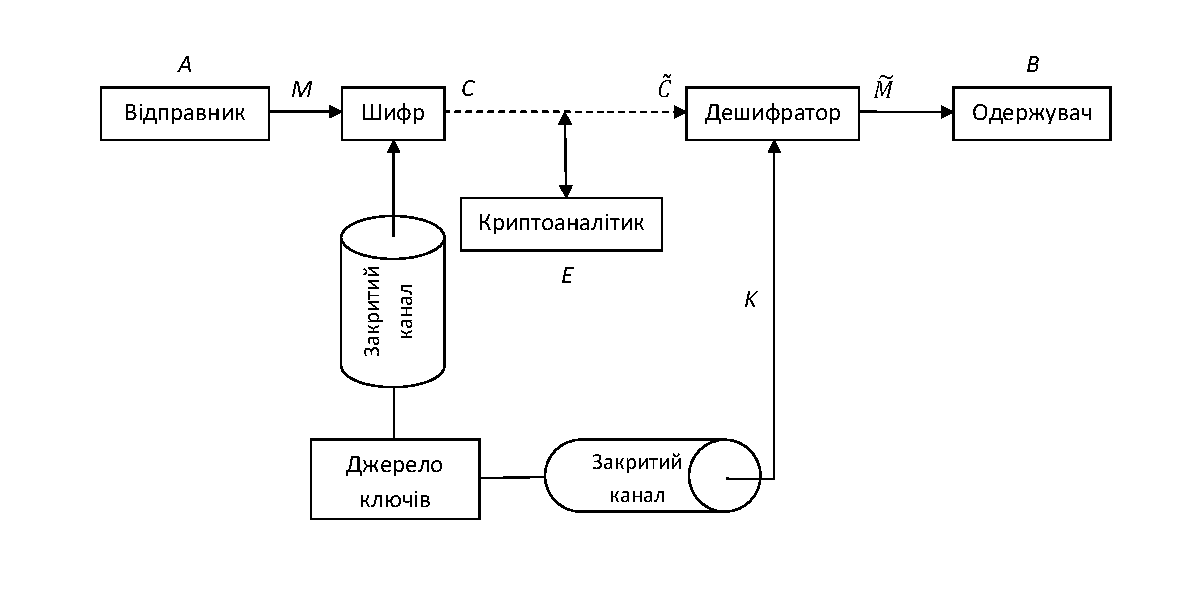
\includegraphics[width=\textwidth]{scheme}
\caption{Загальна схема секретного зв'язку}
\label{im:S_scheme}
\end{figure} 

На рисунку \ref{im:S_scheme}: \textsl{M, C} --
це власне відкритий і шифрований текст;
$\widetilde {M}, \widetilde{C}$ -- якісь змінені ВТ і ШТ відповідно, якщо криптоаналітик \textsl{E} вніс якісь зміни. Зауважимо, що в схемі Шеннона $\textsl {M} = \widetilde{M}$ і $\textsl {C} = \widetilde{C} $. Ну і звісно 
 \textsl{K} є закритим ключем. \par
Пунктирна лінія означає, що передача може бути припинена і передана інформація - змінена.

\begin{center}
Математична модель криптосистеми
\end{center}

З математичної точки зору, криптосистема є сукупністю просторів
\[ \Sigma =  \langle {\mathcal{M},\mathcal{C},\mathcal{K},\mathcal{E},\mathcal{D}} \rangle \, ,\]
\(
\begin{aligned}
\text{де } \mathcal{M} & - \text{простір відкритих текстів}, \\
\mathcal{C} & - \text{простір криптограм}, \\
\mathcal{K} & - \text{простір ключів}, \\
\mathcal{E}  & - \text{простір алгоритмів шифрування}, \\
\mathcal{D} &  - \text{простір алгоритмів розшифрування}.
\end{aligned}
\)  \\ \par
Далі будемо вважати, що $ E_k \in \mathcal{E} $ и $ D_k \in \mathcal{D} $ -- конкретні перетворення, тобто алгоритми шифрування і розшифрування на ключі \textsl {k} відповідно. \par
У загальному випадку під \textsl{шифром} визначається наступне:
\begin{equation}
\text{це відображення} \: \mathcal{M} \times \mathcal{K} \rightarrow \mathcal{C} : \forall{k} \in \mathcal{K}, \textsl{M} \in \mathcal{M} : D_k(E_k(\textsl{M}))=\textsl{M} ,
\end{equation}
 де $E_k : \mathcal{M} \rightarrow \mathcal{C}$ -- ін'єктивне відображення, яке дає можливість зашифрувати будь-який ВТ на ключі \textsl{k}, ну і відповідно при цьому, також відбувається однозначне розшифрування.

\begin{center}
Основні припущення Сіммонса
\end{center}

1. Атака криптоаналітика \textsl{E} здійснюється за допомогою ШТ. \\ \par
Криптоаналітик E хотів би обдурити \textsl {B}, пославши якусь іншу криптограму і щоб він подумав, що це йому відправив \textsl {A}. Якщо така дія вдається \textsl {E}, то вважається, що абонент \textsl {B} введений в оману. \\ \par
2. На декартовому добутку $ \mathcal{M} \times \mathcal {K} $ задано ймовірнісний розподіл. \\ \par

Тобто, така ймовірність \textsl{P(\textsl{M,K})} : $\forall{\textsl{M}} \in \mathcal{M}, \textsl{K} \in \mathcal{K}$ виконується наступне: \\
\[
\sum\limits_{M,K} P(\textsl{M,K}) =1, \;
\sum\limits_{M} P(\textsl{M,K}) = P(\textsl{K}), \;
\sum\limits_{K} P(\textsl{M,K}) = P(\textsl{M}).
\]

Згідно з правилом Керкгоффса, всі простори криптосистеми
$\Sigma$ і розподіл на $ \mathcal{M} \times \mathcal {K} $ вважаються відомими криптоаналітику. \\ \par

Подивимося, як же Сіммонс розвивав свою теорію далі. \\ \par

Він розглянув 2 типи атак: \\ \par
1. \textbf{Імітація}: Криптоаналітик \textsl {E} не очікує справжній ШТ від 
\textsl {A}, тобто не перехоплюючи, формує помилковий ШТ 
$\widetilde {C}$ і відправляє його \textsl {B}. \par
Атака з імітацією вважається успішною, якщо \textsl{B} вважає, що 
$ \widetilde{C} $ допустима криптограма від \textsl {A}, тобто 
$ \widetilde{M} $ -- ВТ, прийнятий за допустимий текст \textsl {A}, навіть якщо \textsl {B} пізніше відправив \\ШТ $ \textsl{C} = \widetilde{C} $. Тобто ця криптограма не розпізнана і в цьому випадку, якщо B був введений в оману, то незалежно від того який там був текст  -- помилковий чи правильний, все одно атака є успішною через те, що криптограма прийшла не в той час, коли відправляв \textsl {A} і відповідно висновки з отриманої криптограми будуть інші. Тому що важливо не тільки зміст криптограми, а й коли вона прийшла.

Позначимо ймовірність імітації :
\begin{equation}  \label{eq:PIM}  
P_{\text{ім}} = \max_{\widetilde{C} \in \mathcal{C}} P(\widetilde{C}- \text{допустима})
\end{equation}
Тобто, щоб обдурити \textsl{B}, криптоаналітик \textsl{E} намагається вибрати таку криптограму $ \widetilde {C} $, щоб максимізувати ймовірність \eqref{eq:PIM}. \\ \par
2. \textbf{Атака підміни}: \textsl{E} перехоплює справжній ШТ \textsl {C} 
від \textsl {A} і формує помилковий ШТ $ \widetilde{C} $ 
і передає його \textsl {B}. \par
Атака вважається успішною, якщо \textsl{B} прийняв $ \widetilde{C} $ за допустиму. \par
Позначимо ймовірність підміни:
\begin{equation}  \label{eq:PSUB}  
P_{\text{підм}} = \max_{\substack{\widetilde{C} \neq \textsl{C} \\
\widetilde{C} \in \mathcal{C}}} P(\widetilde{C} - \text{допустима})
\end{equation} 

Тоді ймовірність обману користувача \textsl{B} буде визначатися так: 
\begin{equation}  \label{eq:PLIE}  
P_{\text{об}} = \max\{P_{\text{ім}},P_{\text{підм}}\}
\end{equation} 

Як визначити систему, яка буде цілком таємною, тобто найкраща з точки зору криптостійкості. То тут цілком природньо було б визначити абсолютно автентичну криптосистему. Але як її визначити, тобто найкращу з точки зору неможливості підробки, обману або такої імітації, не зовсім зрозуміло. І це вже не зовсім тривіальне питання, тому що, якщо передається якесь повідомлення, то така ймовірність обману все одно буде, як ми незабором це побачимо. \\ \par

Проілюструємо загальну схему роботи криптосистеми
на малюнку \eqref {im:S_illustration}. \\
Розглянемо скінченну множину відкритих текстів \textsl{M}, яке зазвичай є певною підмножиною більшої множини і множину шифрованих текстів 
\textsl{C}, яке зазвичай більше за множину ВТ.
Також є множина ключів, яка практично збігається з усім простором ключів, за виключення нетипових слабких ключів. \par
Нехай обрані ключі $ K_1, K_2, K_3 $, на яких працюють абоненти. То ми можемо сказати, що весь простір ВТ відобразиться в деякий підпростір ШТ і позначимо їх $ C_1, C_2, C_3 $ відповідно, які в свою чергу можуть перетинатися, а можуть і не перетинатися.

\begin{figure}[h]
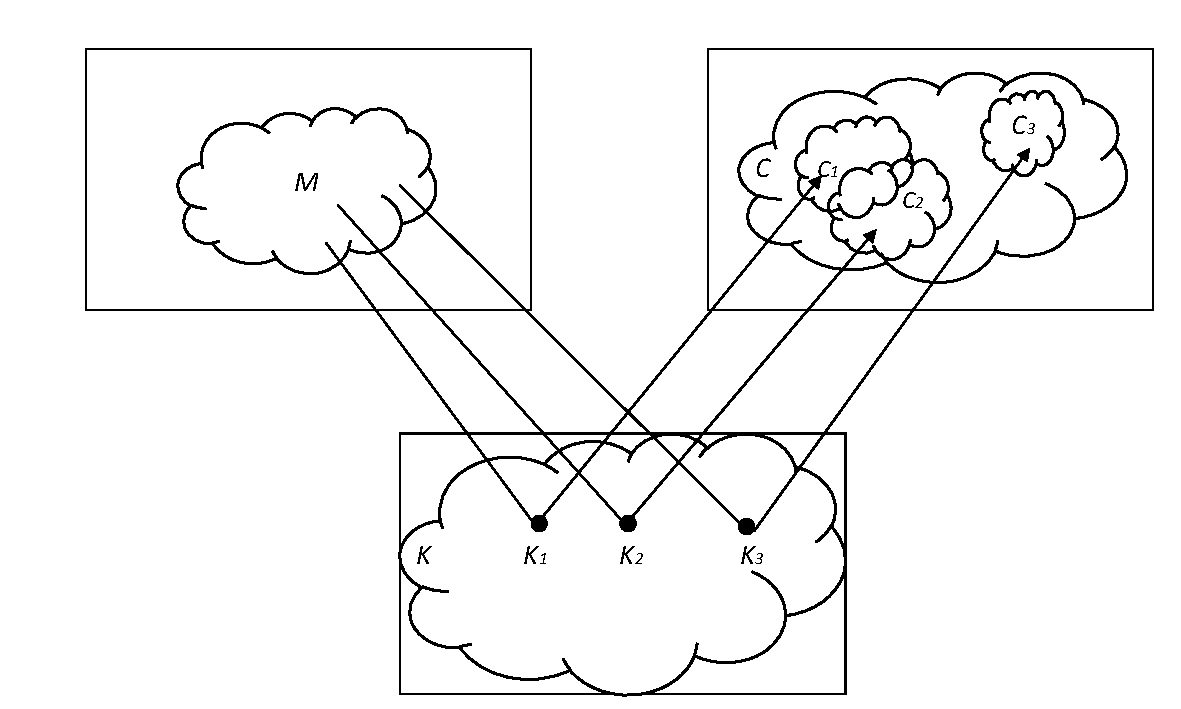
\includegraphics[height=8cm,width=\textwidth,]{illustration}
\caption{Ілюстрація загальної схеми секретного зв'язку}
\label{im:S_illustration}
\end{figure} 
\pagebreak

Розглянемо атаку імітації. \par
Нехай \textsl{A} і \textsl{B} працюють на ключі \textsl{k} і відповідно заданий алгоритм шифрування на цьому ключі:
$E_k(\mathcal{M})=\mathcal{C}_k$, де 
$\mathcal{C}_k \in \mathcal{C}, \textsl{k} \in \mathcal{K}$.   \par
Тоді, якщо абонентами \textsl{A} і 
\textsl{B} вибирається випадкове \textsl{k}, а криптоаналітиком \textsl{E} таке $\widetilde{C} \subset \mathcal{C} $ і відправляє $ \widetilde{C} \rightarrow \textsl{B} $, то ймовірність успіху атаки:
\begin{equation} \label{eq:PIM2}
P(\widetilde{C} - \text{допустима}) = 
\frac{|\mathcal{C}_k|}{|\mathcal{C}|} \geq \frac{|\mathcal{M}|}{|\mathcal{C}|} \textgreater 0,
\end{equation}
причому $|\mathcal{C}_k| \geq |\mathcal{M}| $ через однозначність розшифрування. Також ясно, що $ |\mathcal{M}| \textgreater 0 $. Ну і власне ймовірність \eqref{eq:PIM2} більше нуля, з чого і випливає, що така ймовірність обману існує. \par

В нерівності \eqref{eq:PIM2} досягається рівність $\Leftrightarrow$ 
$\forall \textsl{k} \in \mathcal{K}: |\mathcal{C}_k|=|\mathcal{M}|$, 
\\тобто $\forall{k} \in \mathcal{K}: E_k : \mathcal{M} \rightarrow \mathcal{C}_k$ -- бієкція. \par

Виникає питання, а як же зробити ймовірність обману меншою? \par
Коли застосовуємо до повідомлення цифровий підпис, то фактично ймовірність обману зменшується через те, що збільшується простір ШТ. Далі буде з'ясовано, яким чином вирішити це питання за допомогою імітовставок.

У загальному випадку \textsl{K} вибирається з ймовірністю $P(K)$. \par   
Позначимо через:

\[
        \Ind{K}(\textsl{C\,})=\begin{cases}
                1, &\text{якщо }  \textsl{C} \in \mathcal{C}_K \\
                0, &\text{якщо }  \textsl{C} \notin \mathcal{C}_K
        \end{cases}  - \text{індикатор } \textsl{C},
\] 
тобто $\Ind{K}(\textsl{C\,}) : \mathcal{C} \rightarrow \binsp{} $

Ймовірність того, що $ \widetilde{C} $ -- допустима, визначається наступним:

\begin{equation} \label{eq:P_ALLOWABILITY}
P(\widetilde{C} - \text{допустима}) = 
\sum\limits_{K \in \mathcal{K}} P(\textsl{K}) \cdot \Ind{K}(\widetilde{C})
\end{equation}

Ми не знаємо секретного ключа \textsl{K}, але ми знаємо його розподіл, через що у нас і буде визначена ймовірність \eqref {eq:P_ALLOWABILITY}. Тоді: 
\begin{equation} \label{eq:PIM3}
P_{\text{ім}} = \max_{\substack{\widetilde{C} \in \mathcal{C}}} P(\widetilde{C} - \text{допустима}) =
\max_{\substack{\widetilde{C} \in \mathcal{C}}} 
\sum\limits_{K \in \mathcal{K}} P(\textsl{K}) \cdot \Ind{K}(\widetilde{C}) 
\end{equation}

Шляхом деяких технічних міркувань, з використання нерівності Йєнсена, Сіммонс оцінив ймовірність \eqref{eq:PIM3}:

\begin{equation} \label{eq:P_EVALUATION}
P_{\text{ім}} \geq 2^{-I(\mathcal{C, K})} \:,
\end{equation}
де $I(\mathcal{C, K}) = H(\mathcal{C}) - H(\mathcal{C} | \mathcal{K}) $ -- взаємна інформація. 

При цьому, в нерівності \eqref{eq:P_EVALUATION} рівність досягається 
$\Leftrightarrow$ виконуються наступні умови: \par
1. $P(\widetilde{C} - \text{допустима})$ не залежить від $\widetilde{C}$. Тобто оптимальна атака -- це випадковий вибір криптограми 
$\widetilde{C}$. \par
2. $P(\widetilde{C} | \textsl{K})$ однакова для $\forall \textsl{K} \in \mathcal{K} : \widetilde{C} \in \mathcal{C}_K $, тобто $\Ind{K}(\widetilde{C}) = 1.$

Тоді ймовірність обману визначається наступним:
\begin{equation} \label{eq:PLIECOMMON}
P_{\text{об}} = \max\{P_{\text{ім}},P_{\text{підм}}\} \geq 2^{-I(\mathcal{C, K})} \,.
\end{equation}

\begin{mydef} 
Абсолютно автентичною криптосистемою називається така, для якої в нерівності \eqref{eq:PLIECOMMON} досягається рівність.
\end{mydef}

Ймовірність \eqref{eq:PLIECOMMON} не може бути нульовою, але вона може бути мінімізована, коли взаємна інформація між $ \mathcal{C} $ і 
$ \mathcal{K}$ в свою чергу максимізована. Трактується це наступним чином: наскільки ключ використовується для створення умов імітостійкості. \\ \par

\begin{example}
$\mathcal{M} = \{M_1, M_2\}$ , 
$\mathcal{K} = \{K_1, K_2\}$, 
%$P(K_1) = P(K_2) = \frac{1}{2}, P(M_1) = P(M_2) = \frac{1}{2}$
де кожна подія приймається з однаковою ймовірністю. 
$\mathcal{C}$ = \{00, 01, 10, 11\}.
\end{example} \par  
Задамо алгоритм шифрування у вигляді таблиці \eqref{tab:T1}, при якому показано, якому ШТ відноситься відповідний ВТ на заданому ключі. Також ми подивимось, чи можна зробити ймовірність імітації рівній
 $ \frac{1}{2} $ і яка ж буде ймовірність обману. \\ \par
\begin{wraptable}{l}{0.22\linewidth}
\begin{tabular}{|c||c|c|}\hline
\backslashbox{K}{M}
&\makebox[1.5em]{$M_1$}&\makebox[1.5em]{$M_2$} \\\hline\hline
$K_1$  &00&10 \\ \hline
$K_2$  &01&11 \\ \hline 
\end{tabular} 
        \caption{Алгоритм шифрування}
        \label{tab:T1}
\end{wraptable} 
Однозначність розшифрування в даному прикладі забезпечена, так як видно, що при кожному ключі - ВТ переходить в якийсь відмінний від інших ШТ. \par
Знайдемо взаємну інформацію між $\mathcal{C}$ і $\mathcal{K}$ :
 \begin{equation}
 I(\mathcal{C}, \mathcal{K}) = H(\mathcal{C}) - H(\mathcal{C} | \mathcal{K}) =
  \log(4) - \log(2) = 1 
 \end{equation} 
  
Якщо криптоаналітик посилає якусь довільну криптограму і якщо \textsl{А} і \textsl {B} працюють на ключі $ \textsl{K}_1 $, то він завжди обдурить, якщо вибере один з двох ШТ: 00 або 10. Тобто він з ймовірністю 
$\frac{1}{2}$ зможе здійснити атаку імітації і таким чином в нерівності 
\eqref{eq:P_EVALUATION} досягається рівність. \par
Але чому ж дорівнює ймовірність підміни? \par
Можна помітити, що якщо ключ $ \textsl{K}_1 $, то в криптограмі останній біт -- 0, на ключі $ \textsl{K}_2 $, відповідно -- 1. Таким чином, ми по криптограмі можемо зрозуміти на якому ключі працюють \textsl{А} і 
\textsl{B}, і фактично ця система з точки зору стійкості -- погана. 
Тоді ймовірність підміни буде дорівнювати одиниці, через наступний фактор. Якщо ми перехопимо криптограму 00, то зразу посилаємо 10 і навпаки. 
Ну і звичайно ж ймовірність обману строго більше $  \frac{1}{2} $, 
тобто в \eqref{eq:PLIECOMMON} рівність не досягається. \par
З усього цього слідує те, що наш шифр не є абсолютно автентичним.
Ну і звичайно ж зрозуміло, щоб зменшити ймовірність підміни, необхідно розширювати простір ШТ.
Для цих цілей використовують імітовставки.
\begin{center}
Імітовставки
\end{center}

Нехай $ \textsl{E}_K $ -- алгоритм блочного шифру, а повідомлення 
\textsl{M} розбивається на блоки, \\
тобто $ M = M_1 M_2 \dots M_t $ і в режимі зчеплення блоків при таємному ключі \textsl{K} знаходимо
\begin{equation}
H_i = E_K(M_i \xor H_{i-1}) \:, i=\overline{1,t}
\end{equation}

Розмір блоку дорівнює розміру входу і виходу. тобто
$ |M_i | = |E_K(X)| = |X| $, відповідно \\
$ H_0 $ - вектор ініціалізації, а $ H_t $ - імітовставка. \par
Повідомлення з імітовставкою $ (M, H_t) $ забезпечує автентичність з 
використанням секретного ключа, і при цьому простір отриманих текстів 
розширюється і далі воно може бути зашифровано іншим ключем. Для цієї мети 
також використовуються геш-функції із секретним ключем -- $h(X,K)$.  
\\ \par
Властивості $h(X,K)$:
\begin{enumerate}
\item[1)] Швидке обчислення.
\item[2)] $ \forall M \in \mathcal{M} $ не можна вгадати значення 
геш-функції $h(M,K)$ з ймовірністю більш ніж $ 2^{\min\{m,|K|\}} $, 
де $|K|$ -- довжина ключа в бітах, $m$ -- розмір виходу $h(X,K)$.
\item[3)] Для скінченного набору: $ \{M_i, h(M_i, k) \}_ {i = 1}^ t $ не можливо знайти хоча б одну пару
 $ (M, \widetilde{M}) \: \text {:} \: H(M, k) = h(\widetilde {M}, k) \text{,}\: M \neq \widetilde {M} $ за поліноміальний час.
 
\end{enumerate}
 
Приклад геш-функцій з ключем: імітовставки.

